\documentclass[11pt,a4paper]{article}
\usepackage{fontspec}
\setmainfont{Times New Roman}
\usepackage{textcomp}
\usepackage[left=3.30cm,right=3.651cm,top=2.03cm,bottom=3.05cm,headheight=12pt,headsep=15pt,footskip=30pt]{geometry}
\usepackage{microtype}
\usepackage{booktabs,array,ragged2e}
\usepackage{xcolor}
\usepackage{url}
\usepackage{hyperref}
\usepackage{fancyhdr}
\usepackage{titlesec}
\usepackage{pgfplots}
\pgfplotsset{compat=1.18}
\definecolor{StartColour}{HTML}{283E67}
\definecolor{EndColour}{HTML}{A95234}
\hypersetup{colorlinks=true,urlcolor=StartColour,linkcolor=black,pdfauthor={Uchenna Splendor Ejike, Israel Olanrewaju Odeajo and Goodness Chibueze Kalu.},pdftitle={Path-Robust Risk Controls for Intraday Mean Reversion in NSE Equities}}
\urlstyle{same}
\expandafter\def\expandafter\UrlBreaks\expandafter{\UrlBreaks\do\a\do\b\do\c\do\d\do\e\do\f\do\g\do\h\do\i\do\j\do\k\do\l\do\m\do\n\do\o\do\p\do\q\do\r\do\s\do\t\do\u\do\v\do\w\do\x\do\y\do\z\do\A\do\B\do\C\do\D\do\E\do\F\do\G\do\H\do\I\do\J\do\K\do\L\do\M\do\N\do\O\do\P\do\Q\do\R\do\S\do\T\do\U\do\V\do\W\do\X\do\Y\do\Z\do\0\do\1\do\2\do\3\do\4\do\5\do\6\do\7\do\8\do\9}
\Urlmuskip=0mu plus 1mu\relax
\newcommand{\Needspace}[1]{\par\begingroup\ifdim\dimexpr\pagegoal-\pagetotal\relax<#1\relax\newpage\fi\endgroup}
\setlength{\parindent}{0.43cm}
\setlength{\parskip}{2pt}
\setlength{\emergencystretch}{2em}
\widowpenalty=10000
\clubpenalty=10000
\pagestyle{fancy}
\fancyhf{}
\fancyhead[R]{\fontsize{9}{11}\selectfont Group 17838 | Module 6 Draft Project}
\fancyfoot[R]{\fontsize{9}{11}\selectfont\thepage}
\renewcommand{\headrulewidth}{0pt}
\titleformat{\section}{\normalfont\fontsize{13}{15.6}\selectfont\bfseries}{}{0pt}{}
\titleformat{\subsection}{\normalfont\fontsize{11}{13.2}\selectfont\bfseries}{}{0pt}{}
\titlespacing*{\section}{0pt}{12pt}{6pt}
\titlespacing*{\subsection}{0pt}{9pt}{4pt}
\newlength{\tablecontentwidth}
\setlength{\tabcolsep}{4pt}
\begin{document}
\justifying


\begin{center}{\fontsize{14}{17}\selectfont\bfseries Path\char45{}\allowbreak{}Robust Risk Controls for Intraday Mean Reversion in NSE Equities\par}\vspace{6pt}

\textbf{M6 Draft Project | MScFE 690 Capstone | Student Group 17838}\par\vspace{4pt}

Uchenna Splendor Ejike, Israel Olanrewaju Odeajo and Goodness Chibueze Kalu\par\vspace{4pt}

18 October 2026\par\vspace{4pt}

\end{center}

\begin{center}\bfseries Abstract\end{center}

{\itshape\noindent This project looks at the effectiveness of stop\char45{}\allowbreak{}losses and profit targets to an intraday mean\char45{}\allowbreak{}reversion strategy in five stocks traded on the National Stock Exchange of India. Comparisons are based on identical entries and identical position sizes based on time\char45{}\allowbreak{}only, stop\char45{}\allowbreak{}only and combined exits under stated costs, entry delays and minute\char45{}\allowbreak{}price orderings. The original twenty\char45{}\allowbreak{}session pilot is retained. The number of sessions during an expanded development run is 443, of which 360 (or 381) are evaluable using the two interpretations of the timestamp. The mean returns are lower for combined exits than time\char45{}\allowbreak{}only exits. The development combined\char45{}\allowbreak{}minus\char45{}\allowbreak{}time mean difference nominal 95\% intervals are exploratory and contain zero. Combined exits have lower observed expected shortfall and higher funded drawdown. The two declared candle paths agree on the development reference sample, where no ambiguous episodes occurred. The development notebook introduced funded accounting, two separate drawdowns (one at the minute close and one at the daily close) and paired moving\char45{}\allowbreak{}block intervals. Synthetic diagnostics indicate undercoverage under more pronounced serial dependence. Validation now covers 148 sessions. Combined exits lower mean returns by 0.6885 bp per day under start labels and 0.3855 bp per day under end labels, with lower descriptive expected shortfall but higher funded drawdown. At reference execution, one of 260 end-labelled episodes is ambiguous; the alternative path does not reverse the mean-return ranking. Final testing remains pending. The contribution is a reproducible comparison with submitted exits with explicit data, accounting and inference limits. It does not establish executable profitability.\par}

\section*{Introduction}

The strategy is to be on the buy side when a stock has an unusually poor performance compared to an index, with the hope that it will make up for the shortfall within the next fifteen minutes. A qualifying stock could even have increased in absolute terms, as the index increased by a greater percentage. Stop can end a loss but also can end a position before recovery. A target is a price level that is set to close a trade once a favourable price action occurs, but potentially miss out on future opportunities. So, we compare the exits with the same entry rule to compare them.

The research question is whether stop\char45{}\allowbreak{}only or combined stop\char45{}\allowbreak{}loss and profit\char45{}\allowbreak{}target exits provide greater net returns or less downside risk than fixed\char45{}\allowbreak{}time exits and whether the results hold true under the assumed methods of execution. The primary comparison of Combined vs Time\char45{}\allowbreak{}only exits means the difference in mean daily return. Risk measures and the other policy comparisons focus on different parts of the trade\char45{}\allowbreak{}off. We do not estimate a beta hedge and we do not take up a position on the index; the signal is adjusted with a coefficient of one.

Both exit levels can be present in a minute candle, but it may not be possible to determine which occurred first. It’s also not able to show the spread or available depth or what their order\char39{}s queue priority is. The differences in these gaps are important when determining if an apparent backtest advantage is worth pursuing.

The project keeps the research question submitted in M2 and the scope developed in M4: one entry rule, five stocks, a fifteen-minute holding cap and three exit policies. The original pilot in Tables 5--7 and the expanded development run remain supporting records. This M6 draft develops the methods, results and interpretation without changing those findings. The professor's M4 feedback asked for short explanations connecting the sections and answering why, what, how and what next. The new links between the framework, experiment and discussion address that feedback. The peer review has not yet been received; its comments will be assessed and the responses recorded when it arrives.

\par\addvspace{8pt}\noindent\begin{minipage}{\linewidth}
\textbf{Table 1. Response to feedback and review status}\par\vspace{5pt}
\begingroup\fontsize{9.5}{11.7}\selectfont
\renewcommand{\arraystretch}{1.12}
\setlength{\tablecontentwidth}{\dimexpr\linewidth-2\tabcolsep\relax}
\noindent\begin{tabular}{@{}>{\RaggedRight\arraybackslash}p{0.32\tablecontentwidth}>{\RaggedRight\arraybackslash}p{0.68\tablecontentwidth}@{}}
\toprule
\textbf{Feedback addressed} & \textbf{Response in this draft} \\[3pt]
\midrule
Cuts the scope and does the core & Five fixed development stocks and three exits for one entry rule, extensions after completion of the matched experiment. \\[3pt]
Create original work, and don\char39{}t make a survey & Study specific audit, reproducibility of signals, paired ledgers, ambiguity frequencies and conditional path comparisons; empirical statements are contingent upon a completed replay, and a subsequent final test. \\[3pt]
Update and use appropriate references & The focused framework integrates basic techniques and recent cost\char45{}\allowbreak{}aware intraday research and official calendar evidence. \\[3pt]
Connect the sections and explain the reasoning & Short explanations link the literature to the matched experiment, distinguish risk measures and identify what remains to be tested. \\[3pt]
Body text should be justified. & Justified body paragraphs, readable tables and consistently formatted citations are used throughout the report. \\[3pt]
Peer review & Not yet received. Review comments and the group's responses remain an explicit task before submission. \\[3pt]
\bottomrule\end{tabular}
\endgroup
\end{minipage}\par\addvspace{8pt}

\section*{Theoretical Framework}

\subsection*{Reversal and execution}

However, the reversal in quote\char45{}\allowbreak{}based US returns at the first half\char45{}\allowbreak{}hour lag (9) is the only one that can be statistically confirmed by Heston, Korajczyk and Sadka. Their tried and tested decile techniques end up losing money when trades cross the spread (14). By contrast, de Groot, Huij and Zhou keep the weekly reversion profits after subtracting the estimated costs, varying their stock selection and turnover in their US and European applications (3). These varying outcomes lead us to include implementation in our research question.

Aleti, Bollerslev and Siggaard train, validate and test their models chronologically (7736–37). They claim favorable intraday ETF performance simulations based on their assumptions of spreads and borrowing (7739–40). Their models, their overnight exposure, is different than ours. They do not provide proof of how our stock signal or exit rules will work, but rather they examine costs and timing.

\subsection*{How stopping and targeting can have a positive or negative effect}

Kaminski and Lo demonstrate that the return to a stop overlay is not possible to increase the expected return, under the assumption of independence and identical distribution of returns, and that the risky asset has a positive premium (242). Additionally the mean\char45{}\allowbreak{}reverting AR(1) case yields a first\char45{}\allowbreak{}order return penalty while sufficiently persistent momentum can lead to different results (243–44). The risk that an exit after weakness misses a recovery is relevant adverse evidence. Their rule switches the portfolio exposure and their theoretical treatment assumes that there are no transaction costs (240). It thus does not directly assess our trade barriers.

In Leung and Li\char39{}s stop\char45{}\allowbreak{}constrained Ornstein–Uhlenbeck model, the increase in the stop level decreases the optimal take\char45{}\allowbreak{}profit boundary (15). This illustrates the interaction among the exit rules, not the derivation of thresholds used here. Lo and Remorov demonstrate that some of the more relaxed stops result in gains to the mean variance certainty\char45{}\allowbreak{}equivalent measure or reductions in drawdown and that raw returns are less than would be under the buy and hold strategy (9–10). Risk rankings and return ratings may thus vary. Aggarwal gives an Indian example of comparing pair\char45{}\allowbreak{}trading exits, trading at daily closing prices and day\char45{}\allowbreak{}end execution without spread adjustment (55–57).

These studies give reasons for both gains and losses from early exits. We therefore keep entries and position sizes the same, so the comparison shows what changes when the exit rule changes.

\subsection*{Observation and evaluation}

Maier\char45{}\allowbreak{}Paape and Platen demonstrate that a candle which finally reaches both barriers can leave an active position\char39{}s exit unresolved (17). This known problem is measured in the chosen NSE sample – how frequently it does occur, how this impacts on exit policy comparisons, and which assumptions alter the conclusions.

Sullivan, Timmermann and White describe the processes by which one surviving rule out of many tries can exaggerate evidence of success (1–3). We maintain a single signal, and record each sensitivity run but don\char39{}t apply their Reality Check (5–6). Acerbi and Tasche\char39{}s expected\char45{}\allowbreak{}shortfall definition includes probability mass at the tail edge (5\char45{}\allowbreak{}6, 9\char45{}\allowbreak{}10). Yamai and Yoshiba demonstrate that the precision of estimation is still influenced by the shape of the tail and the size of the sample (89–90, 95–96). Convincing a risk estimate can be difficult even with a correct calculation.

The evidence does not establish that this NSE signal or these barriers will be profitable. It defines what the experiment must separate: the effect of the exit rule, the assumptions used for execution, and the uncertainty in the reported estimates.

\section*{Methodology}

\subsection*{Conventions used for samples and data}

The frozen pilot is using RELIANCE, HDFCBANK, INFY, TCS and ITC with the provided .NSEI between 1 January\char45{}\allowbreak{}31 March 2021. To make it manageable, we fixed these five names beforehand, before the observation of strategy outcomes. The notebook keeps them in a study calendar for 1 January 2021 – 31 December 2023. Parsing a later file does not imply that its strategy outcomes have been evaluated, source preparation and strategy evaluation is done separately. History of spreads and depths cannot be established based on available activity measures for this sample. The results are specific to the stocks and dates analyzed.

On the NSE calendar, 26 January, 11 March and 29 March are marked as first\char45{}\allowbreak{}quarter holidays on weekdays, which leaves 61 trading dates in the first quarter of the year (National Stock Exchange of India, “Trading Holidays for the Calendar Year 2021”). The Securities and Exchange Board of India (SEBI) have noted the 24 February suspension and the extended session (1–2). It also says NSE submitted that NIFTY computation was unavailable between 10:06 and 11:43 (8). These sources describe the event, but do not prove that our files are complete.

The pilot does not include the full day of 24th February and keeps this day as missing history. The next 20 sessions are also barred under the rule and eligibility can be restored from 26 March. This will intentionally dispose of all otherwise useable windows on 24 February. We fixed the restriction before computing P\&L for pilots, but the trader would not have been able to know about the event beforehand. The exclusion does not give any indication of loss per outage day nor a minimum performance.

We have assumed 09:15 – 15:30 Asia/Kolkata time and are studying both start and end labelled minutes, pending supplier confirmation. We don\char39{}t select an interpretation for better returns. The parser supports explicit input dates in the form MM/DD/YYYY and DD\char45{}\allowbreak{}MM\char45{}\allowbreak{}YYYY, and rejects any other date format, invalid OHLC and time non\char45{}\allowbreak{}minute format. In\char45{}\allowbreak{}month timestamps have to be strictly increasing and duplicate keys are rejected. An out\char45{}\allowbreak{}of\char45{}\allowbreak{}month row is only excluded from the result set by a documented exception if the timestamp matches an already retained row from the original monthly source and all OHLCV values are identical. The ingestion stops if there are unmatched or conflicting rows. Verified copies have a separate count of exclusions, while all source rows are included in the audit count and in the parsed\char45{}\allowbreak{}content digest. Raw files are not altered. The limits are some corporate actions, some historical charges, tick sizes and source metadata is not yet resolved.

The 5 stocks selected had 1,883 copied observations in their September 2023 cash files dated 22 August 2023. Every one of these corresponds to the same August time stamp and OHLCV values: RELIANCE, HDFCBANK and TCS – 377 copies each, INFY and ITC – 376 copies each. These copies appear in the loader, but as verified copies, are not changed and are excluded by the loader. No observations were available for this date (22 September 2023) in the selected cash files; August prices are not used to reconstruct this date. The rules for feature\char45{}\allowbreak{}history and outcome\char45{}\allowbreak{}identification as declared above remain valid for missing data. This is a finding related to the quality of the sources, not to the actual performance of the final period strategy.

\subsection*{Signals and corresponding exits}

We subtract the log return from the completed 15\char45{}\allowbreak{}minute interval for the index from the log return for the stock during the same interval at each decision time. We determine the z value of this difference based on the mean and sample standard deviation of differences for the same clock time in the twenty scheduled sessions that immediately precede the session that contains it. The calculation is not valid if history is missing or if it has zero variance. Valid dates that are older than the window cannot be used to fill in missing dates in the window.

Under start labels, a 09:45 decision uses the log of the close labelled 09:44 / close labelled 09:29. All sixteen consecutive bars must be on both instruments. Then end labels are shifted back 1 minute and the same calculation is applied. Decisions are taken every 30 minutes after 30 minutes of the session begins. A z score of −2 or lower allows for a long position at the beginning price one minute later. The full 15\char45{}\allowbreak{}minute holding window must fit within the session.

Define P as the entry price, and let v be the sample standard deviation of the stock\char39{}s own same\char45{}\allowbreak{}clock 15\char45{}\allowbreak{}minute log returns for those 20 sessions. The stop is P × exp(\char45{}\allowbreak{}v) and the target is P × exp(1.5v). These are fixed, non\char45{}\allowbreak{}trailing points that continue the design that has been submitted. The signal is based on relative weakness and the distances of the barriers are based on the volatility of the stock. The z\char45{}\allowbreak{}value is not a calibrated probability and the barriers are not estimates of the optimal exit level.

\par\addvspace{8pt}\noindent\begin{minipage}{\linewidth}
\textbf{Table 2. Matched exit policies}\par\vspace{5pt}
\begingroup\fontsize{9.5}{11.7}\selectfont
\renewcommand{\arraystretch}{1.12}
\setlength{\tablecontentwidth}{\dimexpr\linewidth-2\tabcolsep\relax}
\noindent\begin{tabular}{@{}>{\RaggedRight\arraybackslash}p{0.32\tablecontentwidth}>{\RaggedRight\arraybackslash}p{0.68\tablecontentwidth}@{}}
\toprule
\textbf{Policy} & \textbf{Exit rule} \\[3pt]
\midrule
Time\char45{}\allowbreak{}only & Close at common scheduled expiry. \\[3pt]
Stop\char45{}\allowbreak{}only & At that expiry unless closed at the stop. \\[3pt]
Stop and target & Close on the first barrier triggered otherwise at the expiry. \\[3pt]
\bottomrule\end{tabular}
\endgroup
\end{minipage}\par\addvspace{8pt}

For every delay scenario, all policies share the same entries, allocations and expiry. Each entry uses 0.5 × C0 / N: INR 10,000 for five stocks and reference capital C0 of INR 100,000. The research positions are on a fractional share basis and have a maximum of one position per stock. Early exit proceeds are kept aside until the common expiry time. It is a design which compares exits on the same opportunities, without separately optimising each strategy, or having the ability to exit early to fund further trading.

\subsection*{Rationale and limitations of fixed design}

A manageable case study is assured through the five stock universe, implementation and audit work. It is not a random sample nor a recorded order of historical liquidity nor can it reflect the entire exchange. Keeping the same names will prevent changing the sample based on the results.

Comparisons are made at the same clock time with 20 scheduled sessions of history representing approximately one trading month. This is NOT an empirically best lookback, but a short reference window. The threshold of \char45{}\allowbreak{}2 for z scores is not a calibrated tail probability, but an unusually low index\char45{}\allowbreak{}adjusted return given that window. One illustrative asymmetric pair in log\char45{}\allowbreak{}price space is between the 1v stop and 1.5v target. Not necessarily assumed to be optimal or to provide a realised reward\char45{}\allowbreak{}to\char45{}\allowbreak{}risk ratio. Reference cost and checks of 15 bp and 5/25 bp respectively are assumed but not validated historical rates.

These explanations are included post\char45{}\allowbreak{}development and serve to explain the current design. They do not show a previously undocumented selection process. No change of the parameters or selected stocks because of the findings.

\subsection*{Execution and costs}

Minute prices show the range traded, but they do not always show which barrier was reached first. We compare both stated price paths and count the trades for which this uncertainty matters.

The engine uses open\char45{}\allowbreak{}low\char45{}\allowbreak{}high\char45{}\allowbreak{}close and open\char45{}\allowbreak{}high\char45{}\allowbreak{}low\char45{}\allowbreak{}close paths in a uniform manner for all policies. When the active long position\char39{}s candle opens between the barriers and touches both, then these paths create stop first and target first results. These are not recovered ticks, but possible sequences, nor are they universal drawdown bounds. Opening price dictates the exit at scheduled expiry before any subsequent candle tops or bottoms. Prior to the expiration, an opening gap through the stop will fill at the open with the specified adverse slippage. No price improvement and gap above the target fills at the target. A threshold touch is still an assumed fill.

The reference round trip cost is 15 bps of entry notional with 1/2 at entry and 1/2 at exit. We change one assumption at a time; total cost to 5 or 25 bp, extra stop slippage to 5 or 10 bp, or entry delay of two or five minutes. The same fixed charge cancels when matched policy returns are subtracted, but this does affect a policy\char39{}s absolute return. The actual charges according to exit value are not required to cancel. These checks focus on selected execution assumptions and do not provide checks for all sources of spread, market\char45{}\allowbreak{}impact or fill risk.

\subsection*{The amount estimated and accounting}

Each pilot day starts independently with C0. The main estimate is the average delta P\&L of fixed\char45{}\allowbreak{}notional sessions over C0, for those dates for which all the required signals and all policy outcomes are measurable. If one of the required signals cannot be calculated, the entire day\char39{}s primary comparison won\char39{}t be available; this is not the same as a valid signal that results in no trade. This estimate is also conditional on a complete case, and on the basis of this, the independent\char45{}\allowbreak{}session comparison was also performed. It outlines the evaluable dates, but not performance on every date and the viability of cash between dates.

These rules are implemented in the notebook after the frozen pilot and before validation or final\char45{}\allowbreak{}test strategy outcomes are examined. The funded diagnostic will record an abstention if pre\char45{}\allowbreak{}entry signal information is unavailable. If a bar doesn\char39{}t provide an entry/exit value or held position value, then the outcome is unknown, not that there was no trade. Diagnostics make it possible to differentiate between abstentions, valid no\char45{}\allowbreak{}trade days, incomplete primary coverage, unresolved outcomes and funding failures. Funded diagnostics do not substitute an alternative sample for the primary complete\char45{}\allowbreak{}case sample.

A separate feasibility investigation is done for funded accounting. C0 is always the starting reference capital for each call to development, validation and final\char45{}\allowbreak{}test. In that diagnostic, cash and realised P\&L are carried over days, notionals stay fixed and costs are charged on fills. There is no reinvestment of the gains and borrowing is not allowed. The matched funded comparison is stopped when the first economic funding failure occurs. Record keeps date, account affected, available cash and known equity, required funding with fees. An exit\char45{}\allowbreak{}fee cash deficit also puts an end to the comparison. The previous funded path is descriptive, since its endpoint depends on outcomes and it is not a substitute for the main fixed\char45{}\allowbreak{}calendar comparison. A failure cannot be deleted or followed by a cash reset within that funded segment.

If one does not know the market price when confirming an equity account, a cash amount is known, and the account has no open positions, then missing market prices need not interrupt its equity record. Unresolved post entry P\&L does break the funded record until resolved. Starting new days later with independent money can\char39{}t make up for an unknown funded cash balance. A gap is not a place where a new cash reset is allowed in the same funded segment. If there is a separately reported restart with prior P\&L not reconciled, the restart must be labeled as a new independent segment with explicit initial conditions and cannot be connected with the wealth path before the restart.

Equity includes cash and open positions marked to market. Drawdown measures are reported separately for saved minute\char45{}\allowbreak{}close and known\char45{}\allowbreak{}flat boundary marks and for completed daily closes in the notebook. Both start at the beginning of the recorded segment capital. The identified closing cash of levelled\char45{}\allowbreak{}out finished funded sessions is daily\char45{}\allowbreak{}close equity. If a partial mark is part of an interrupted day, it is not a daily close. If no identified day is completed in a segment the statistics for the daily\char45{}\allowbreak{}close are not available, and separate segments are never joined. Fixed\char45{}\allowbreak{}capital normalisation is P\&L divided by C0, not a return on changing opening wealth. ES97.5 is the Mean of the worst 2.5\% of daily losses (fractional cut\char45{}\allowbreak{}off weighting). The independent-session accounts use common evaluable dates across policies; each policy\char39{}s ES is calculated separately on those dates prior to subtraction. Funded drawdown is its own sample and endpoint – ES is descriptive. Here, independent-session describes a daily capital reset, not statistical independence between dates. Neither frequency of valuation identifies losses hidden within the minute.

\subsection*{Evaluation rules and completion plan}

The main comparison is the combined\char45{}\allowbreak{}minus\char45{}\allowbreak{}time mean net daily return at reference costs, entry delay and stop\char45{}\allowbreak{}first ordering. The hypothesis of no difference is the null hypothesis. Secondary comparison: Stop\char45{}\allowbreak{}minus\char45{}\allowbreak{}time, combined\char45{}\allowbreak{}minus\char45{}\allowbreak{}stop. Combined\char45{}\allowbreak{}minus\char45{}\allowbreak{}stop is an indicator of how much the target adds to the selected stop. There is no target\char45{}\allowbreak{}only policy or estimate of the total stop–target interaction.

The 60/20/20 split is based on the full period calendar, not just the dates that meet the complete\char45{}\allowbreak{}case requirements. In this case, we have n sessions planned: development stops at session floor(0.60n), validation stops at session floor(0.80n), and final test runs on the rest of the sessions. The recorded boundaries are 1 January 2021–17 October 2022, 18 October 2022–25 May 2023 and 26 May 2023–29 December 2023, based on 739 normal sessions. The calendar covers the holiday amendment (National Stock Exchange of India, “Trading Holidays for the Calendar Year 2022”; National Stock Exchange of India, “Trading Holidays for the Calendar Year 2023”; NSE Clearing Limited) made in June 2023. Validation was completed on 18 October 2026; final-test strategy outcomes remain unevaluated. Later exclusions cannot move these boundaries. Features could be initialised from past observations. Validation may result in the discovery of bugs or corrections for metadata based on independent evidence, but not for undocumented searches for more favourable thresholds, stocks or exclusions. Amendments will be noted prior to final testing and the original pilot and any test results already observed will be retained.

The notebook is based on a nominal 95\% paired moving\char45{}\allowbreak{}block percentile interval with 2000 repetitions and seed 17838. The five day blocks are primary blocks, the ten and twenty day blocks are sensitivities. Whole paired daily observations are sampled within each contiguous eligible calendar segment. Blocks are sampled uniformly with replacement and concatenated to the original segment length, with the exception of the sampled block of the end which is truncated. No original date is removed from the point estimate. If any segment has length smaller than the length of its block or if \(\sum_j \lfloor L_j / b\rfloor < 10\), then the interval is withheld. Here \(L_j\) is the number of eligible sessions in segment \(j\), and \(b\) is the block length in sessions. This support rule does not guarantee independence, coverage or power, it is only a reporting threshold. It is an adaptation of fixed\char45{}\allowbreak{}block resampling to the observed gaps (Künsch) and does not retrieve missing outcomes. The development update includes synthetic reliability and interval\char45{}\allowbreak{}width diagnostics in addition to market results. Group review of validation and final freezing of the protocol remain pending. Block lengths must not be selected for significance.

All of the currently nominal 95\% bootstrap intervals are exploratory. Interval not including zero indicates the direction according to the assumed resampling model, but not a statistically reliable effect. Synthetic diagnostics indicate under coverage. Additional repetitions or selection of a favourable block length do not resolve that limitation. Such restriction shall be for development, validation and final outputs of the present procedure. Sensitivity tests illustrate the results\char39{} sensitivity to the assumptions made. There is a trade\char45{}\allowbreak{}off between lower sampled risk and lower returns.

This exploratory status must be maintained with the protocol review or a separately specified inferential amendment must be documented and evaluated before final outcomes are accessed. That assessment must consider the following: dependence and missing\char45{}\allowbreak{}date patterns, interval coverage and width, and simulation uncertainty. If there is no supporting evidence for defensibility, then descriptive effect estimates and exploratory intervals will be retained in the final report. The software checks or the saving of a protocol freeze does not create statistical reliability.

Sample size expansion may not make tail\char45{}\allowbreak{}risk estimates sufficiently precise. The fixed final partition has 148 scheduled sessions, or the equivalent of up to 3.70 days of scheduled ES97.5 tail weight (without exclusions). This is not an actual final\char45{}\allowbreak{}test sample; it is a Calendar calculation. Unless supported by documented precision assessment, final ES will be descriptive. The notebook shows the actual number of samples, the tail dates and tail leave\char45{}\allowbreak{}one\char45{}\allowbreak{}day\char45{}\allowbreak{}out sensitivities for each stage performed. Independent tail events cannot be formed with more trades or bootstrap repetitions.

\par\addvspace{8pt}\noindent\begin{minipage}{\linewidth}
\textbf{Table 3. Current stage of implementation and remaining gates.}\par\vspace{5pt}
\begingroup\fontsize{9.5}{11.7}\selectfont
\renewcommand{\arraystretch}{1.12}
\setlength{\tablecontentwidth}{\dimexpr\linewidth-2\tabcolsep\relax}
\noindent\begin{tabular}{@{}>{\RaggedRight\arraybackslash}p{0.32\tablecontentwidth}>{\RaggedRight\arraybackslash}p{0.68\tablecontentwidth}@{}}
\toprule
\textbf{Stage} & \textbf{Status / required evidence} \\[3pt]
\midrule
Inherited pilot and development evidence & Completed historical records. Tables 5--10 and their original run identifiers are retained. These are not new M6 market runs. \\[3pt]
M6 report development & Explanatory links, source corrections and the dated working plan have been added. The M4 feedback is addressed; peer review is pending. \\[3pt]
M6 notebook checks & Independent trade, cash, day and episode reconciliation, chronological boundary checks and runtime package recording are implemented. All 25 code cells completed, 111 local software tests passed, and all 14 market ledger reconciliations passed. The scope of these checks is stated in Appendix B. \\[3pt]
Source and metadata resolution & Verified copied rows remain audited. Timestamp meaning, adjustment conventions and execution metadata remain unresolved where supplier evidence is unavailable. \\[3pt]
Validation & Completed on 18 October 2026: all 148 scheduled sessions are evaluable under both timestamp interpretations in all seven settings. Results and manifests are retained separately from development. \\[3pt]
Final evaluation & The 26 May--29 December 2023 final strategy outcomes remain unevaluated. Final evaluation and protocol freezing are disabled in the interim M6 notebook. \\[3pt]
\bottomrule\end{tabular}
\endgroup
\end{minipage}\par\addvspace{8pt}

\subsection*{Group working plan}

Table 4 gives the remaining group work for the M6 deadline of 3 November 2026 at 00:00 GMT (01:00 in Berlin). The internal completion target is 2 November, allowing time to check the files. These are planned responsibilities and dates, not claims that each task has already been completed. Final-test access remains outside this interim release until validation review and a documented protocol freeze are complete.

\par\addvspace{8pt}\noindent\begin{minipage}{\linewidth}
\textbf{Table 4. Group working plan to the M6 deadline}\par\vspace{5pt}
\begingroup\fontsize{9.5}{11.7}\selectfont
\renewcommand{\arraystretch}{1.12}
\setlength{\tablecontentwidth}{\dimexpr\linewidth-4\tabcolsep\relax}
\noindent\begin{tabular}{@{}>{\RaggedRight\arraybackslash}p{0.25\tablecontentwidth}>{\RaggedRight\arraybackslash}p{0.17\tablecontentwidth}>{\RaggedRight\arraybackslash}p{0.58\tablecontentwidth}@{}}
\toprule
\textbf{Work and lead} & \textbf{Target} & \textbf{Completion evidence} \\[3pt]
\midrule
Code and reconciliation: Uchenna & 18--22 Oct. & Review and reproduce the validation run completed on 18 October; verify its manifests, ledger checks and recorded limitations. \\[3pt]
Data review: Israel & 18--23 Oct. & Review source counts, exclusions, calendar boundaries and outstanding metadata. Keep both timestamp interpretations where unresolved. \\[3pt]
Analysis and references: Goodness & 23--27 Oct. & Check each table against saved results; explain the findings and limitations; verify citations and update the reference list. \\[3pt]
Peer feedback: all members & On receipt; review by 28 Oct. & Assess each received comment and record the response. If unavailable, record that status and seek the instructor's direction. \\[3pt]
Draft review: all members & 28--30 Oct. & Check the research question, method, results and conclusion for agreement; confirm the remaining tasks and interpretation limits. \\[3pt]
Reproduction and file checks: all members & 31 Oct.--1 Nov. & Reproduce the submitted outputs, verify figures and units, inspect the PDF and confirm that the supporting files open correctly. \\[3pt]
Group sign-off and upload & 2 Nov. & Complete the group review and provide the PDF separately from the supporting ZIP before the course deadline. \\[3pt]
\bottomrule\end{tabular}
\endgroup
\end{minipage}\par\addvspace{8pt}

While timestamp conventions remain unconfirmed, we retain both conditional interpretations. In cases of sparse coverage, inference may not be available. Where ambiguous episodes are absent, we report this absence, but do not modify barriers to manufacture dual hits.

\section*{Results}

The pilot and development findings establish the starting evidence for M6. The new validation results follow them in a separate subsection. Dates and run identifiers distinguish the three stages; their samples are not pooled.

\subsection*{Frozen pilot: implementation and coverage}

The original M4 pilot added streamed ingestion, strict parser, past only signals and session accounting to M3. Independent calculations verified the reported signals, executions and daily accounts in that version which passed 99 checks. These are historical checks tables 5\char45{}\allowbreak{}7, not current notebook test count or proof of historical fills. Later, self\char45{}\allowbreak{}contained notebooks and verification records are detailed in the dev update and Appendix A. The code can be found in the link: \url{https://github.com/I-am-Uchenna/nse-intraday-risk-controls}.

The frozen pilot sample includes 137,036 rows from eighteen monthly files that are held by the instructor in the NSE Cash Stocks Data and NSE Index Data. These selected rows were successful in the pilot parser checks and missing intervals were left in. This is the count of the original Q1 sample. The later source audit commands its own manifest and is not able to certify instruments and files beyond the study inputs selected.

\par\addvspace{8pt}\noindent\begin{minipage}{\linewidth}
\textbf{Table 5. Session / Episode coverage of reference execution settings}\par\vspace{5pt}
\begingroup\fontsize{9.5}{11.7}\selectfont
\renewcommand{\arraystretch}{1.12}
\setlength{\tablecontentwidth}{\dimexpr\linewidth-4\tabcolsep\relax}
\noindent\begin{tabular}{@{}>{\RaggedRight\arraybackslash}p{0.52\tablecontentwidth}>{\RaggedRight\arraybackslash}p{0.24\tablecontentwidth}>{\RaggedRight\arraybackslash}p{0.24\tablecontentwidth}@{}}
\toprule
\textbf{Measure} & \textbf{Start labels} & \textbf{End labels} \\[3pt]
\midrule
Scheduled Q1 sessions & 61 & 61 \\[3pt]
Initial history\char45{}\allowbreak{}only sessions & 20 & 20 \\[3pt]
Nonstandard session excluded & 1 & 1 \\[3pt]
Subsequent sessions with an incomplete prior history & 20 & 20 \\[3pt]
Common evaluable sessions & 20 & 20 \\[3pt]
Valid zero\char45{}\allowbreak{}trade sessions: & 4 & 7 \\[3pt]
Unique eligible trade episodes. & 33 & 24 \\[3pt]
Unresolved episodes & 0 & 0 \\[3pt]
Ambiguous episodes of active dual\char45{}\allowbreak{}barrier (ADB) & 0 & 0 \\[3pt]
\bottomrule\end{tabular}
\endgroup
\par\smallskip{\small\noindent From Frozen M4 replay \char45{}\allowbreak{} results/m4\_pilot/summary.json Twenty evaluable dates are available: 1–23 February (seventeen sessions), 26 March, 30 March and 31 March. Label interpretations change signals and entries, counts are unique episodes and not repeated policy/path accounts.\par}
\end{minipage}\par\addvspace{8pt}

\subsection*{Conditional comparisons}

\par\addvspace{8pt}\noindent\begin{minipage}{\linewidth}
\textbf{Table 6. Reference mean daily P\&L / reference capital, in basis points}\par\vspace{5pt}
\begingroup\fontsize{9.5}{11.7}\selectfont
\renewcommand{\arraystretch}{1.12}
\setlength{\tablecontentwidth}{\dimexpr\linewidth-4\tabcolsep\relax}
\noindent\begin{tabular}{@{}>{\RaggedRight\arraybackslash}p{0.52\tablecontentwidth}>{\RaggedRight\arraybackslash}p{0.24\tablecontentwidth}>{\RaggedRight\arraybackslash}p{0.24\tablecontentwidth}@{}}
\toprule
\textbf{Policy and/or paired contrast} & \textbf{Start labels} & \textbf{End labels} \\[3pt]
\midrule
Time\char45{}\allowbreak{}only & \char45{}\allowbreak{}2.914 & \char45{}\allowbreak{}0.886 \\[3pt]
Stop\char45{}\allowbreak{}only & \char45{}\allowbreak{}2.734 & \char45{}\allowbreak{}1.359 \\[3pt]
Stop and target & \char45{}\allowbreak{}3.476 & \char45{}\allowbreak{}1.957 \\[3pt]
Combined minus time & \char45{}\allowbreak{}0.562 & \char45{}\allowbreak{}1.072 \\[3pt]
Stop minus time & +0.180 & \char45{}\allowbreak{}0.473 \\[3pt]
Combined minus stop & \char45{}\allowbreak{}0.742 & \char45{}\allowbreak{}0.598 \\[3pt]
\bottomrule\end{tabular}
\endgroup
\par\smallskip{\small\noindent Means and paired contrasts produced from scenario\_means.csv and paired\_contrasts.csv. The default settings are 15 bp round trip, no additional stop slippage and a 1 minute entry delay. Each day starts independently with capital of INR 100,000 with each basis point being INR 10. Both paths agree because no active episode encounters both barriers in one candle.\par}
\end{minipage}\par\addvspace{8pt}

\par\addvspace{8pt}\noindent\begin{minipage}{\linewidth}
\textbf{Table 7. Sensitivity (bps of reference capital) in paired mean daily differences}\par\vspace{5pt}
\begingroup\fontsize{9.5}{11.7}\selectfont
\renewcommand{\arraystretch}{1.12}
\setlength{\tablecontentwidth}{\dimexpr\linewidth-8\tabcolsep\relax}
\noindent\begin{tabular}{@{}>{\RaggedRight\arraybackslash}p{0.26\tablecontentwidth}>{\RaggedRight\arraybackslash}p{0.185\tablecontentwidth}>{\RaggedRight\arraybackslash}p{0.185\tablecontentwidth}>{\RaggedRight\arraybackslash}p{0.185\tablecontentwidth}>{\RaggedRight\arraybackslash}p{0.185\tablecontentwidth}@{}}
\toprule
\textbf{Setting} & \textbf{Start: combined\char45{}\allowbreak{}time} & \textbf{Start: stop\char45{}\allowbreak{}time} & \textbf{End: combined\char45{}\allowbreak{}time} & \textbf{End: stop\char45{}\allowbreak{}time} \\[3pt]
\midrule
Reference & \char45{}\allowbreak{}0.562 & +0.180 & \char45{}\allowbreak{}1.072 & \char45{}\allowbreak{}0.473 \\[3pt]
Common cost 5 bp & \char45{}\allowbreak{}0.562 & +0.180 & \char45{}\allowbreak{}1.072 & \char45{}\allowbreak{}0.473 \\[3pt]
Common cost 25 bp & \char45{}\allowbreak{}0.562 & +0.180 & \char45{}\allowbreak{}1.072 & \char45{}\allowbreak{}0.473 \\[3pt]
Stop slippage +5 bp & \char45{}\allowbreak{}0.962 & \char45{}\allowbreak{}0.220 & \char45{}\allowbreak{}1.297 & \char45{}\allowbreak{}0.698 \\[3pt]
Stop slippage +10 bp & \char45{}\allowbreak{}1.362 & \char45{}\allowbreak{}0.620 & \char45{}\allowbreak{}1.522 & \char45{}\allowbreak{}0.923 \\[3pt]
Entry delay 2 min & \char45{}\allowbreak{}0.071 & +0.476 & \char45{}\allowbreak{}1.204 & \char45{}\allowbreak{}0.641 \\[3pt]
Entry delay 5 min & \char45{}\allowbreak{}0.997 & +0.027 & \char45{}\allowbreak{}1.466 & \char45{}\allowbreak{}0.667 \\[3pt]
\bottomrule\end{tabular}
\endgroup
\par\smallskip{\small\noindent Data from paired\_contrasts.csv and sensitivity\_comparisons.csv. Each setting have exactly the same twenty evaluable dates. Entries need not be preserved in case of delay and/or label changes. Common fixed costs are eliminated in the comparisons and absolute returns continue to vary. For instance, end\char45{}\allowbreak{}label time\char45{}\allowbreak{}only has an average of +0.314 bp per day at a 5 bp cost, whereas stop\char45{}\allowbreak{}only and combined are still negative.\par}
\end{minipage}\par\addvspace{8pt}

At the reference cost, all three policies lose, on average. Combined exits do not perform as well as time\char45{}\allowbreak{}only in all the stated settings. The small stop\char45{}\allowbreak{}only advantage of the start\char45{}\allowbreak{}label becomes negative with the addition of 5 bp stop slippage. The result has been obtained by the development pilot. In the case of 20 equally weighted daily outcomes, empirical ES97.5 would be the same as the worst observed loss. Hence, the pilot does not report any ES, drawdown, Sharpe ratio or inferential interval.

\section*{Expanded development results}

\subsection*{Completed scope and data audit}

Notebook run 20261001T221531Z\char45{}\allowbreak{}th2hk303 evaluated 1 January 2021–17 October 2022 under code \nolinkurl{8b40cf6e4170a157095ecfc28d0579cf1299c99a} and protocol SHA\char45{}\allowbreak{}256 \nolinkurl{c6363f28828d9ab3080556ff887ea6c58501a462883bc792a4272495518bc39b}. It has the original 5 stocks, entry rule and 3 exits. It ran 14 cost/delay \& timestamp scenarios – these are not independent experiments but related. A total of 216 selected monthly files were prepared and 1,669,406 unique rows were retained from 1 January 2021 until 31 December 2023. Those source dates extend beyond the evaluated development partition. This is the declared source window for six series, and not a statement of minute a minute coverage, nor an audit of every instrument delivered. This leaves the June 2023 supplement, which has not yet been reconciled, outside of the sample. This development record contains no validation or final-test strategy outcomes; the new validation run is reported separately below.

The source audit records the verified 1,883 August copies and also the missing cash information for 22 September 2023. The hosted development run was successful, with all 24 code cells completed without errors. The M4 revision passed 104 software tests and a second cached\char45{}\allowbreak{}pilot run reproduces all 84 historical policy/scenario means to within a maximum of 0.000000000001 bp. These computation checks are useful for being able to reproduce results under the assumptions. They are not evidence of historical execution quality.

\subsection*{Independent\char45{}\allowbreak{}session estimates}

\par\addvspace{8pt}\noindent\begin{minipage}{\linewidth}
\textbf{Table 8. In the reference execution, an expanded development comparison is performed.}\par\vspace{5pt}
\begingroup\fontsize{9.5}{11.7}\selectfont
\renewcommand{\arraystretch}{1.12}
\setlength{\tablecontentwidth}{\dimexpr\linewidth-4\tabcolsep\relax}
\noindent\begin{tabular}{@{}>{\RaggedRight\arraybackslash}p{0.52\tablecontentwidth}>{\RaggedRight\arraybackslash}p{0.24\tablecontentwidth}>{\RaggedRight\arraybackslash}p{0.24\tablecontentwidth}@{}}
\toprule
\textbf{Measure} & \textbf{Start labels} & \textbf{End labels} \\[3pt]
\midrule
Scheduled development sessions & 443 & 443 \\[3pt]
Common evaluable independent sessions & 360 & 381 \\[3pt]
Mean daily P\&L / C0 (bp) \char45{}\allowbreak{} time only & \char45{}\allowbreak{}2.3362 & \char45{}\allowbreak{}2.3863 \\[3pt]
Stop\char45{}\allowbreak{}only mean daily P\&L / C0 (bp) & \char45{}\allowbreak{}2.5925 & \char45{}\allowbreak{}2.4935 \\[3pt]
Combined mean daily P\&L / C0 (bp) & \char45{}\allowbreak{}2.5687 & \char45{}\allowbreak{}2.5137 \\[3pt]
Combined minus time (bp). & \char45{}\allowbreak{}0.2325 & \char45{}\allowbreak{}0.1273 \\[3pt]
Primary five-day exploratory 95\% interval (bp) & [\char45{}\allowbreak{}0.4410, 0.0770] & [\char45{}\allowbreak{}0.3269, 0.1299] \\[3pt]
Time\char45{}\allowbreak{}only ES97.5 daily loss (bp). & 17.4085 & 15.3083 \\[3pt]
Daily loss (bp) for the stop\char45{}\allowbreak{}only group (ES97.5) & 14.8495 & 14.2981 \\[3pt]
Daily ES97.5 loss (bp) for combined exits & 14.4075 & 13.2774 \\[3pt]
The tail mass (days) of the ES97.5. & 9.000 & 9.525 \\[3pt]
Unique ambiguous / eligible episodes. & 0 / 637 & 0 / 662 \\[3pt]
\bottomrule\end{tabular}
\endgroup
\par\smallskip{\small\noindent Data source: This run\char39{}s policy\_means.csv, paired\_effects.csv, expected\_shortfall.csv, intervals.csv and exit\_ambiguity.csv. Reference execution: 15 bp round\char45{}\allowbreak{}trip cost, one\char45{}\allowbreak{}minute delay and no extra stop slippage and O\char45{}\allowbreak{}L\char45{}\allowbreak{}H\char45{}\allowbreak{}C ordering. Means and ES: common independent\char45{}\allowbreak{}session days, missing outcomes are not zero returns. The intervals are still exploratory. Any interval that includes 0 (including when an endpoint is 0) is inconclusive. ES is descriptive. These development observations are not final tests and are not intended as a substitute for the original pilot.\par}
\end{minipage}\par\addvspace{8pt}

All the main intervals of combined\char45{}\allowbreak{}minus\char45{}\allowbreak{}time are still exploratory and also have a zero under either of the two timestamp interpretations. Combined exits have lower mean returns, as well as lower observed ES97.5, than time\char45{}\allowbreak{}only exits. It\char39{}s descriptive risk\char45{}\allowbreak{}return trade\char45{}\allowbreak{}off, not evidence of a better exit policy. The ES tail includes just 9.000 or 9.525 days of probability mass, with tail dates and leave\char45{}\allowbreak{}one\char45{}\allowbreak{}day\char45{}\allowbreak{}out ranges given with the output. For combined\char45{}\allowbreak{}minus\char45{}\allowbreak{}time, both the five\char45{}\allowbreak{}day primary and ten\char45{}\allowbreak{}day sensitivity intervals include zero. 20\char45{}\allowbreak{}day intervals are not taken due to the fact that the first eligible segment is 17 days. Because no reference\char45{}\allowbreak{}scenario episode on the common evaluable dates hits both barriers, identical path outcomes do not establish robustness with respect to an unobserved ambiguity.

% image_alt: "Development execution sensitivity"

% image_destination: "output/colab/aligned_development/development_sensitivity_print.png"

\par\addvspace{8pt}\noindent\begin{minipage}{\linewidth}

\centering
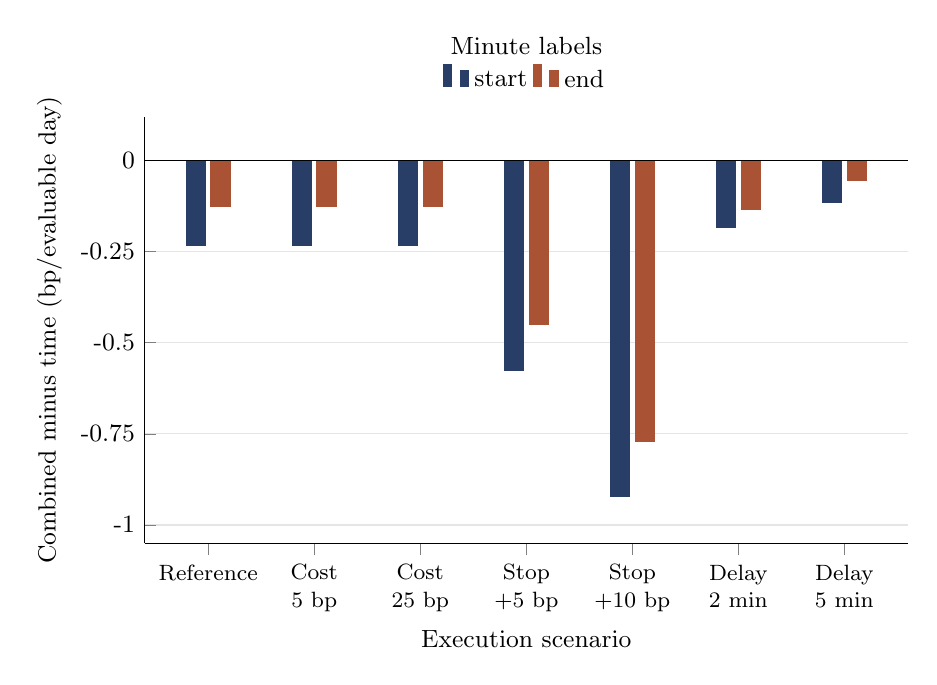
\begin{tikzpicture}
\begin{axis}[
width=0.93\linewidth,height=7cm,
ybar,bar width=7pt,
xmin=-0.6,xmax=6.6,ymin=-1.05,ymax=0.12,
xtick={0,1,2,3,4,5,6},
xticklabels={{Reference},{Cost\\5 bp},{Cost\\25 bp},{Stop\\+5 bp},{Stop\\+10 bp},{Delay\\2 min},{Delay\\5 min}},
x tick label style={font=\fontsize{8.5}{10}\selectfont,align=center},
y tick label style={font=\small},
ytick={-1,-0.75,-0.5,-0.25,0},
yticklabels={{\char45{}\allowbreak{}1},{\char45{}\allowbreak{}0.75},{\char45{}\allowbreak{}0.5},{\char45{}\allowbreak{}0.25},{0}},
scaled y ticks=false,
ylabel={Combined minus time (bp/evaluable day)},
ylabel style={align=center,font=\small},
xlabel={Execution scenario},xlabel style={font=\small},
ymajorgrids=true,grid style={gray!20},
axis x line*=bottom,axis y line*=left,
legend style={at={(0.5,1.03)},anchor=south,draw=none,font=\small},
legend columns=2,legend entries={{start},{end}},
title={Minute labels},title style={font=\small,yshift=13pt},
]
\addplot[fill=StartColour,draw=StartColour] coordinates {(0,-0.23247870094142048) (1,-0.23247870094142042) (2,-0.2324787009414204) (3,-0.5769231453858609) (4,-0.9213675898303175) (5,-0.18401247913573263) (6,-0.11507160284811925)};
\addplot[fill=EndColour,draw=EndColour] coordinates {(0,-0.12732863740261363) (1,-0.12732863740261363) (2,-0.12732863740261363) (3,-0.44885094711391504) (4,-0.7703732568251972) (5,-0.13599521891106853) (6,-0.05515904296995816)};
\draw[black,thin] (axis cs:-0.6,0)--(axis cs:6.6,0);
\end{axis}
\end{tikzpicture}

\par\smallskip{\small\RaggedRight Figure 1. Combined minus time mean effects for the declared execution scenarios. The following comparisons are aligned on reference and stressed dates within each interpretation of the timestamps. The Y axis is basis points (bps) of reference capital per evaluable day. The figures plotted are point estimates, not confidence intervals, and these are development comparisons.\par}

\end{minipage}\par\addvspace{8pt}

\subsection*{In two observation frequencies there is funded equity.}

\par\addvspace{8pt}\noindent\begin{minipage}{\linewidth}
\textbf{Table 9. Funded drawdown in development under execution of the reference.}\par\vspace{5pt}
\begingroup\fontsize{9.5}{11.7}\selectfont
\renewcommand{\arraystretch}{1.12}
\setlength{\tablecontentwidth}{\dimexpr\linewidth-8\tabcolsep\relax}
\noindent\begin{tabular}{@{}>{\RaggedRight\arraybackslash}p{0.23\tablecontentwidth}>{\RaggedRight\arraybackslash}p{0.22\tablecontentwidth}>{\RaggedRight\arraybackslash}p{0.21\tablecontentwidth}>{\RaggedRight\arraybackslash}p{0.14\tablecontentwidth}>{\RaggedRight\arraybackslash}p{0.2\tablecontentwidth}@{}}
\toprule
\textbf{Minute labels / policy} & \textbf{Maximum drawdown (\%) at minute and boundary marks} & \textbf{Daily\char45{}\allowbreak{}close maximum drawdown (\%)} & \textbf{Identified daily closes} & \textbf{The most recent date with an identified daily close.} \\[3pt]
\midrule
Start: Time\char45{}\allowbreak{}only & 9.4282 & 9.3359 & 443 & 2022\char45{}\allowbreak{}10\char45{}\allowbreak{}17 \\[3pt]
Start: Stop\char45{}\allowbreak{}only & 10.4371 & 10.3714 & 443 & 2022\char45{}\allowbreak{}10\char45{}\allowbreak{}17 \\[3pt]
Start: Combined & 10.1413 & 10.1191 & 443 & 2022\char45{}\allowbreak{}10\char45{}\allowbreak{}17 \\[3pt]
End: Time\char45{}\allowbreak{}only & 9.9072 & 9.8252 & 443 & 2022\char45{}\allowbreak{}10\char45{}\allowbreak{}17 \\[3pt]
End: Stop\char45{}\allowbreak{}only & 10.1650 & 10.0845 & 443 & 2022\char45{}\allowbreak{}10\char45{}\allowbreak{}17 \\[3pt]
End: Combined & 10.0296 & 10.0116 & 443 & 2022\char45{}\allowbreak{}10\char45{}\allowbreak{}17 \\[3pt]
\bottomrule\end{tabular}
\endgroup
\par\smallskip{\small\noindent Source: funded\_drawdown.csv, O\char45{}\allowbreak{}L\char45{}\allowbreak{}H\char45{}\allowbreak{}C reference accounts. The six accounts shown each contain one identified segment within its timestamp interpretation in the time range, 1 January 2021 to 17 October 2022. None of the funded accounts are early ending; there are 443 identified daily closes for each account. The beginning of each segment begins at its recorded C0. The maximum drawdown at minute marks includes all the saved marks and does not include the downsampling plotting. Daily\char45{}\allowbreak{}close drawdown is based on finished, identified sessions and an independent daily\char45{}\allowbreak{}close peak. There is no requirement for the independent\char45{}\allowbreak{}session day count in the funded sample, where there are known abstentions. A failure or unidentified position may end the minute record during a day, after the last daily close. Equity between multiple segments cannot be joined; initial conditions for each segment need to be identified.\par}
\end{minipage}\par\addvspace{8pt}

Under both interpretations of the timestamp and for both valuation frequencies, both of the stop\char45{}\allowbreak{}based policies exhibit a higher funded maximum drawdown than time\char45{}\allowbreak{}only. Reducing independent\char45{}\allowbreak{}session ES is not necessarily a reduction in funded drawdown. Additional identified abstention days and trades permitted when other candidate information is unavailable are included in the funded diagnostic. It has a different sample and cash path compared to the primary complete\char45{}\allowbreak{}case comparison.

\subsection*{Calculating and interpreting bootstraps.}

The added diagnostics use the specified resampler on Gaussian paired daily differences with mean 0 and stationary standard deviation 1 bp: independent observations and AR(1) coefficients 0.3 and 0.7. Each process evolves over all 443 of the scheduled development dates before the actual 360 day or 381 day eligibility mask is applied. These diagnostics evaluate repeated\char45{}\allowbreak{}sample interval coverage and width for these specified processes, in addition to arithmetic tests. The experiment is carried out using 200 simulated samples per design, the settings of the experiment, the seed and the output are reported in bootstrap\_reliability.csv. This is a zero mean coverage experiment, no power is claimed on a trading advantage.

\par\addvspace{8pt}\noindent\begin{minipage}{\linewidth}
\textbf{Table 10. Synthetic bootstrap diagnostics}\par\vspace{5pt}
\begingroup\fontsize{9.5}{11.7}\selectfont
\renewcommand{\arraystretch}{1.12}
\setlength{\tablecontentwidth}{\dimexpr\linewidth-6\tabcolsep\relax}
\noindent\begin{tabular}{@{}>{\RaggedRight\arraybackslash}p{0.28\tablecontentwidth}>{\RaggedRight\arraybackslash}p{0.24\tablecontentwidth}>{\RaggedRight\arraybackslash}p{0.28\tablecontentwidth}>{\RaggedRight\arraybackslash}p{0.2\tablecontentwidth}@{}}
\toprule
\textbf{Mask and AR(1) coefficient} & \textbf{Coverage \%, MCSE pp} & \textbf{Average width bp, MCSE bp} & \textbf{Mean / oracle width (ratio)} \\[3pt]
\midrule
Start, AR(1) 0.0 & 90.5 (2.07) & 0.1993 (0.0010) & 0.965 \\[3pt]
End, AR(1) 0.0 & 94.5 (1.61) & 0.1964 (0.0010) & 0.978 \\[3pt]
Start, AR(1) 0.3 & 91.0 (2.02) & 0.2530 (0.0015) & 0.902 \\[3pt]
End, AR(1) 0.3 & 89.0 (2.21) & 0.2485 (0.0014) & 0.910 \\[3pt]
Start, AR(1) 0.7 & 78.5 (2.90) & 0.3368 (0.0025) & 0.696 \\[3pt]
End, AR(1) 0.7 & 81.5 (2.75) & 0.3334 (0.0024) & 0.705 \\[3pt]
\bottomrule\end{tabular}
\endgroup
\end{minipage}\par\addvspace{8pt}

Coverage ranges from 78.5\% to 94.5\%. At a AR(1) coefficient of 0.7, they are respectively 78.5\% for start labels and 81.5\% for end labels. Even for these simple stationary processes, the nominal 95\% procedure can thus be undercover. The table gives Monte Carlo standard errors (not confidence limits) in parentheses. For each design, the 200 intervals from independent histories are available in each row, the 2,000 re\char45{}\allowbreak{}samples per interval, and 5 day blocks. The exact Gaussian width calculated from the known covariance and retained dates is also compared with the mean width. The process seed is 20261002; the bootstrap seed is 17838. The histories shared between the two masks are simulated, and are not independent experiments per row. This diagnostic was set up after the original development run and prior to validation or final\char45{}\allowbreak{}test evaluation. This is not a retroactive pre\char45{}\allowbreak{}registration. Caching arithmetic is able to reproduce the original interval function on three paired probe vectors for each mask within 1e\char45{}\allowbreak{}11 bp. These checks are based on the observed masks and fixed bootstrap seed. They do not model missingness depending on some outcome, heavy tails, regime change, nor do they provide coverage for the true NSE process or recover omitted dates. Unsupported market intervals are still not available. We report undercoverage as a limitation, and don\char39{}t choose a \char34{}block length\char34{} after looking at the effect. Group review of validation and the final freeze remain pending.

\subsection*{M6 validation: fixed design on later sessions}

The validation run completed on 18 October 2026 with the same five stocks, entry rule, barriers and execution settings. It evaluates 18 October 2022--25 May 2023. All 148 scheduled sessions are evaluable under both timestamp interpretations in every setting. The 216 selected source files were read again from the instructor's Drive archives, retaining 1,669,406 rows after the same 1,883 verified duplicate exclusions. Their parsed-data fingerprint matches the development record. Final-period source preparation remains distinct from strategy evaluation: final-test outcomes were not evaluated.

\par\addvspace{8pt}\noindent\begin{minipage}{\linewidth}
\textbf{Table 11. Validation returns and risk at reference execution}\par\vspace{5pt}
\begingroup\fontsize{9.5}{11.7}\selectfont
\renewcommand{\arraystretch}{1.12}
\setlength{\tablecontentwidth}{\dimexpr\linewidth-8\tabcolsep\relax}
\noindent\begin{tabular}{@{}>{\RaggedRight\arraybackslash}p{0.25\tablecontentwidth}>{\RaggedRight\arraybackslash}p{0.16\tablecontentwidth}>{\RaggedRight\arraybackslash}p{0.16\tablecontentwidth}>{\RaggedRight\arraybackslash}p{0.225\tablecontentwidth}>{\RaggedRight\arraybackslash}p{0.205\tablecontentwidth}@{}}
\toprule
\textbf{Labels / exit} & \textbf{Mean (bp/day)} & \textbf{ES97.5 (bp)} & \textbf{Minute / boundary MDD (\%)} & \textbf{Daily-close MDD (\%)} \\[3pt]
\midrule
Start / Time & -2.0100 & 13.3647 & 3.0080 & 2.9851 \\[3pt]
Start / Stop & -2.2864 & 11.6941 & 3.4170 & 3.3891 \\[3pt]
Start / Combined & -2.6985 & 11.8599 & 4.0344 & 4.0140 \\[3pt]
End / Time & -2.0510 & 13.9353 & 3.0476 & 3.0354 \\[3pt]
End / Stop & -2.4511 & 11.8667 & 3.6397 & 3.6276 \\[3pt]
End / Combined & -2.4365 & 12.0332 & 3.6181 & 3.6060 \\[3pt]
\bottomrule\end{tabular}
\endgroup
\end{minipage}\par\addvspace{8pt}

Table 11 uses 15 bp round-trip costs, a one-minute entry delay and O-L-H-C ordering. Mean daily P\&L and ES are normalised by INR 100,000. Each ES has only 3.70 days of effective tail weight; the worst three daily losses receive full weight and the fourth receives 0.70. The funded accounts also have 148 identified daily closes, with no economic funding failure. The accounting remains different even though the date counts now agree. Drawdowns measure saved marks, not unseen intraminute extremes.

The combined-minus-time mean difference is \(-0.6885\) bp per day under start labels and \(-0.3855\) bp under end labels. The nominal five-day-block 95\% intervals are [\(-1.7037\), \(-0.0809\)] and [\(-1.2170\), 0.1695] bp, respectively. The first excludes zero, but both remain exploratory because of the documented coverage limitation. Ten-day-block intervals are [\(-1.7444\), \(-0.0607\)] and [\(-1.2630\), 0.1873] bp. Twenty-day intervals are withheld: 148 sessions provide only seven support blocks, below the declared minimum of ten. This absence is a reporting rule, not a failed notebook cell.

Both stop-based exits have lower descriptive ES than time-only exits, but lower mean returns and larger funded drawdowns. Adding a target to the stop changes the mean by \(-0.4120\) bp under start labels and +0.0146 bp under end labels. Those mixed signs do not support a general benefit from the target. The combined-exit ES leave-one-day-out range is 11.2186--11.8669 bp under start labels and 11.4182--12.0384 bp under end labels. These are sensitivity ranges, not confidence intervals.

\par\addvspace{8pt}\noindent\begin{minipage}{\linewidth}
\textbf{Table 12. Validation execution sensitivity}\par\vspace{5pt}
\begingroup\fontsize{9.5}{11.7}\selectfont
\renewcommand{\arraystretch}{1.12}
\setlength{\tablecontentwidth}{\dimexpr\linewidth-4\tabcolsep\relax}
\noindent\begin{tabular}{@{}>{\RaggedRight\arraybackslash}p{0.5\tablecontentwidth}>{\RaggedRight\arraybackslash}p{0.25\tablecontentwidth}>{\RaggedRight\arraybackslash}p{0.25\tablecontentwidth}@{}}
\toprule
\textbf{One changed assumption} & \textbf{Start labels (bp/day)} & \textbf{End labels (bp/day)} \\[3pt]
\midrule
Reference & -0.6885 & -0.3855 \\[3pt]
5 bp round-trip cost & -0.6885 & -0.3855 \\[3pt]
25 bp round-trip cost & -0.6885 & -0.3855 \\[3pt]
Extra stop slippage: 5 bp & -1.0838 & -0.7335 \\[3pt]
Extra stop slippage: 10 bp & -1.4790 & -1.0815 \\[3pt]
Entry delay: 2 minutes & -0.2592 & -0.2919 \\[3pt]
Entry delay: 5 minutes & -0.4418 & -0.1920 \\[3pt]
\bottomrule\end{tabular}
\endgroup
\end{minipage}\par\addvspace{8pt}

Table 12 reports combined minus time in bp of reference capital per day, using O-L-H-C and the same 148 dates for every row. The contrast remains negative in all seven settings. Equal fixed-notional fees cancel in the paired comparison by construction; this is not evidence of general cost robustness. An additional 10 bp stop penalty reduces the contrast by 0.7905 bp under start labels and 0.6959 bp under end labels. Delayed entries change the comparison and its barriers, but do not reverse its sign.

Unlike development, validation contains one reference ambiguous episode under end labels: 1 of 260 (0.3846\%). At reference execution, start labels have none among 266 episodes. For end labels, the combined mean is \(-2.4365\) bp under O-L-H-C and \(-2.4093\) bp under O-H-L-C, a difference of 0.0272 bp per day. The combined-minus-time contrast changes from \(-0.3855\) to \(-0.3583\) bp; both are negative. One stop exit becomes a target exit. These episode counts describe reference execution only: start-labelled two- and five-minute delays also produce path differences, each about 0.0239 bp per day. This is limited evidence of the effect of candle ordering in the declared sample, not enough to establish broad path robustness or the actual historical execution sequence.

Run \nolinkurl{20261018T084332Z-ghd27dnw} records these outputs. All 25 code cells completed without stored Python errors after the Drive connection was established, and the saved code cells match the checked local source. All 14 ledger reconciliations passed the INR $10^{-7}$ tolerance; the largest recorded discrepancy is below INR $2.73\times10^{-11}$. Repeated policy, path and accounting records are not independent observations. The checks establish internal arithmetic consistency within their stated scope, not real fills, reliable interval coverage or profitability.


\section*{Discussion}

A lower expected shortfall answers a different question from a lower drawdown. We report both and explain their samples and accounting before judging whether an exit policy improves risk.

Evidence of the extended development does not support a mean\char45{}\allowbreak{}return benefit for combined stop\char45{}\allowbreak{}loss and profit target exits. Combined exits result in lower per evaluable day basis points than time\char45{}\allowbreak{}only exits under start\char45{}\allowbreak{} and end\char45{}\allowbreak{}labelled minutes, respectively, by 0.2325 and 0.1273 basis points. This is based on 443 scheduled sessions with 360 and 381 complete case sessions. Lower mean returns also are achieved in all declared cost, slippage and delay settings when combined exits are made. The nominal intervals are exploratory due to synthetic diagnostics showing undercoverage. In their mean\char45{}\allowbreak{}reverting model (243–44), Kaminski and Lo give reasons why a stop may miss a recovery. We find that our result is consistent with that worry, but do not identify their mechanism, as their portfolio overlay isn\char39{}t the same as ours, and we haven\char39{}t estimated their return model.

Development execution sensitivities are used to understand the policy comparison. Combined\char45{}\allowbreak{}minus\char45{}\allowbreak{}time difference is worsened by 0.6889 bp and 0.6430 bp under start and end labels, respectively, for the 10 bp stop slippage. The difference becomes less negative with a 5\char45{}\allowbreak{}minute delay by 0.1174 and 0.0722 bp, but it does not change the sign of the difference. Matched contrasts in the stated fee model cancel the common fixed charges, but not the absolute returns. Delay and timestamp changes can modify entries and barriers – these scenarios do not isolate causal effects with trades held constant. The preceding 20 day pilot is a compendious record of implementation. Its small stop\char45{}\allowbreak{}only advantage is not successful in an added\char45{}\allowbreak{}slippage check.

Reduction of expected shortfall does not prove that the overall risk is reduced. ES reports the mean of the worst 2.5\% of daily losses on common evaluable independent\char45{}\allowbreak{}session dates. Funded drawdown features a distinct cash path with extra days and trades identified in development. In validation, both accounting samples cover the same 148 dates, but their definitions still differ. The funded drawdowns for both stop\char45{}\allowbreak{}based policies are larger than time\char45{}\allowbreak{}only for both valuation frequencies reported. This divergence cannot be attributed to metric alone, due to various risks quantities, accounting and sample. Lo and Remorov also report that the rankings of stop policies vary depending on the type of return or risk measure being considered (9–10), which does not predict our specific ranking. However, here, negative mean returns, lower descriptive ES and larger funded drawdowns do not establish overall superiority.

The candle ambiguity problem is already set by Maier\char45{}\allowbreak{}Paape and Platen (17). In the development sample, there are no eligible reference episodes with common evaluable dates that touch both barriers within one active candle: the observed counts are 0/637 and 0/662. Both the two declared paths thus agree on this sample. These counts are not population limits nor form any sort of robustness when faced with ambiguous candles. The study provides a reproducible comparison of the submitted exits with explicit limits on execution, missingness and inference. Synthetic both\char45{}\allowbreak{}hit cases test implementation, rather than the historical significance of ambiguity. The policy outcomes, paired contrasts, common coverage, ambiguity counts and exit reasons will be carried over to the final report. The validation results above add one ambiguous end-labelled episode; final evaluation remains pending.

The outage\char45{}\allowbreak{}day exclusion illustrates the potential limitation of the sample by the complete\char45{}\allowbreak{}case rule. It removes a stressful session and has an impact on subsequent regular dates in the historical window. Notebook diagnostics differentiate between deliberate exclusions and unavailable features, as well as those that were not captured post\char45{}\allowbreak{}entry and economic funding failures; a coverage audit captures gaps from sources. Complete case estimates can be either over or under estimated. We will be reporting their conditional scope instead of performance on the entire calendar.

\par\addvspace{8pt}\noindent\begin{minipage}{\linewidth}
\textbf{Table 13. Obstacles and responses}\par\vspace{5pt}
\begingroup\fontsize{9.5}{11.7}\selectfont
\renewcommand{\arraystretch}{1.12}
\setlength{\tablecontentwidth}{\dimexpr\linewidth-2\tabcolsep\relax}
\noindent\begin{tabular}{@{}>{\RaggedRight\arraybackslash}p{0.32\tablecontentwidth}>{\RaggedRight\arraybackslash}p{0.68\tablecontentwidth}@{}}
\toprule
\textbf{Obstacle} & \textbf{Response and remaining limit} \\[3pt]
\midrule
Unconfirmed interval labels or time zone & Compare both interpretations for diagnostics, seek confirmation from the source and hold back final claims which are dependent on the timing. \\[3pt]
Deliveries overlapping or conflicting with other deliveries. & Maintain the source identity, only removing copies which are known to be identical and out of month. Any rows that are unmatched or have conflicts will prevent the ingestion. \\[3pt]
Missing intervals and sessions not held at the usual time & Do not backfill any gaps or forward fill prices; retain exclusions and missing history, and do not silently select complete trades. \\[3pt]
Unknown spreads, impact and actual fills & Use declared cost/fill scenarios; do not claim executable returns or capacity. \\[3pt]
Limited days for independent assessments & Describe estimates, present intervals as exploratory until coverage and tail precision have been evaluated. \\[3pt]
Funded\char45{}\allowbreak{}record interruption & Keep the first failure or unknown outcome and its prefix; never concatenate unreconciled segments. \\[3pt]
\bottomrule\end{tabular}
\endgroup
\end{minipage}\par\addvspace{8pt}

This record can be used by researchers to make a decision whether or not to further investigate the selected exit controls. The same audit method can be used to audit broker or platform backtests, where the results of bracket\char45{}\allowbreak{}orders rely on a candle sequence that isn\char39{}t disclosed. Other markets may have researchers who can modify the approach to their respective calendars, instruments and costs. There is no evidence of performance in those markets which is provided by the NSE results themselves.

\section*{Conclusion}

The development and validation comparisons do not show a mean return advantage from adding the chosen stop and target to fixed time exits. The results do not demonstrate overall superiority as lower descriptive expected shortfall is associated with lower mean returns and higher funded drawdown. The two declared candle paths agree on the development reference sample. At reference execution, validation adds one ambiguous end-labelled episode; its alternative ordering changes the combined return but not its ranking below time-only exits. The three-exit question and fixed design of the project are kept. The work now offers matched comparisons, funded accounting and explicit checks of the reliability of its inference. Group review, the remaining feedback, protocol review and final evaluation are pending. Data conventions and assumed execution limit interpretation; a completed backtest does not certify actual fills or profitability.

\section*{References}

{\RaggedRight\hangindent=1.27cm\hangafter=1\noindent Acerbi, Carlo, and Dirk Tasche. “On the Coherence of Expected Shortfall.” \textit{arXiv}, version 5, 2 May 2002, \url{https://arxiv.org/abs/cond-mat/0104295v5}.\par}\vspace{5pt}

{\RaggedRight\hangindent=1.27cm\hangafter=1\noindent Aggarwal, Geetu. \textit{A Study of Statistical Arbitrage Opportunities in Indian Securities Market}. 2021. Punjab Agricultural University, PhD dissertation. \textit{Krishikosh}, \url{https://krishikosh.egranth.ac.in/server/api/core/bitstreams/357e6dad-9c6a-45ca-8329-991561dd3a66/content}.\par}\vspace{5pt}

{\RaggedRight\hangindent=1.27cm\hangafter=1\noindent Aleti, Saketh, et al. “Intraday Market Return Predictability Culled from the Factor Zoo.” \textit{Management Science}, vol. 71, no. 9, 2025, pp. 7731--51, \url{https://doi.org/10.1287/mnsc.2023.01657}.\par}\vspace{5pt}

{\RaggedRight\hangindent=1.27cm\hangafter=1\noindent de Groot, Wilma, et al. “Another Look at Trading Costs and Short-Term Reversal Profits.” Accepted manuscript, July 2011. \textit{Erasmus University Rotterdam}, \url{https://repub.eur.nl/pub/25718/AnotherLook_2011.pdf}.\par}\vspace{5pt}

{\RaggedRight\hangindent=1.27cm\hangafter=1\noindent Heston, Steven L., et al. “Intraday Patterns in the Cross-Section of Stock Returns.” \textit{arXiv}, version 1, 19 May 2010, \url{https://arxiv.org/abs/1005.3535v1}.\par}\vspace{5pt}

{\RaggedRight\hangindent=1.27cm\hangafter=1\noindent Kaminski, Kathryn M., and Andrew W. Lo. “When Do Stop-Loss Rules Stop Losses?” \textit{Journal of Financial Markets}, vol. 18, 2014, pp. 234--54, \url{https://doi.org/10.1016/j.finmar.2013.07.001}.\par}\vspace{5pt}

{\RaggedRight\hangindent=1.27cm\hangafter=1\noindent Künsch, Hans R. “The Jackknife and the Bootstrap for General Stationary Observations.” \textit{The Annals of Statistics}, vol. 17, no. 3, 1989, pp. 1217--41, \url{https://doi.org/10.1214/aos/1176347265}.\par}\vspace{5pt}

{\RaggedRight\hangindent=1.27cm\hangafter=1\noindent Leung, Tim, and Xin Li. “Optimal Mean Reversion Trading with Transaction Costs and Stop-Loss Exit.” \textit{arXiv}, version 3, 14 May 2015, \url{https://arxiv.org/abs/1411.5062v3}.\par}\vspace{5pt}

{\RaggedRight\hangindent=1.27cm\hangafter=1\noindent Lo, Andrew W., and Alexander Remorov. “Stop-Loss Strategies with Serial Correlation, Regime Switching, and Transaction Costs.” \textit{Journal of Financial Markets}, vol. 34, 2017, pp. 1--15, \url{https://doi.org/10.1016/j.finmar.2017.02.003}.\par}\vspace{5pt}

{\RaggedRight\hangindent=1.27cm\hangafter=1\noindent Maier-Paape, Stanislaus, and Andreas Platen. “Backtest of Trading Systems on Candle Charts.” \textit{IFTA Journal}, 2016, pp. 10--17, \url{https://www.ifta.org/assets/docs/d_ifta_journal_16.pdf}.\par}\vspace{5pt}

{\RaggedRight\hangindent=1.27cm\hangafter=1\noindent National Stock Exchange of India. “Trading Holidays for the Calendar Year 2021.” Circular NSE/CMTR/46623, 11 Dec. 2020, \url{https://archives.nseindia.com/content/circulars/CMTR46623.pdf}. Accessed 30 Sept. 2026.\par}\vspace{5pt}

{\RaggedRight\hangindent=1.27cm\hangafter=1\noindent National Stock Exchange of India. “Trading Holidays for the Calendar Year 2022.” Circular NSE/CMTR/50560, 10 Dec. 2021, \url{https://archives.nseindia.com/content/circulars/CMTR50560.pdf}. Accessed 2 Oct. 2026.\par}\vspace{5pt}

{\RaggedRight\hangindent=1.27cm\hangafter=1\noindent National Stock Exchange of India. “Trading Holidays for the Calendar Year 2023.” Circular NSE/CMTR/54757, 8 Dec. 2022, \url{https://archives.nseindia.com/content/circulars/CMTR54757.pdf}. Accessed 2 Oct. 2026.\par}\vspace{5pt}

{\RaggedRight\hangindent=1.27cm\hangafter=1\noindent \textit{NSE Cash Stocks Data}. 2021--2023. Unpublished minute-level data provided by the instructor for MScFE 690 Capstone, WorldQuant University. Accessed locally 30 Sept. 2026.\par}\vspace{5pt}

{\RaggedRight\hangindent=1.27cm\hangafter=1\noindent NSE Clearing Limited. “Changes in Settlement Schedule on Account of Holiday on June 29, 2023.” Circular NCL/CMPT/57291, 27 June 2023, \url{https://archives.nseindia.com/content/circulars/CMPT57291.pdf}. Accessed 2 Oct. 2026.\par}\vspace{5pt}

{\RaggedRight\hangindent=1.27cm\hangafter=1\noindent \textit{NSE Index Data}. 2021--2023. Unpublished minute-level data provided by the instructor for MScFE 690 Capstone, WorldQuant University. Accessed locally 30 Sept. 2026.\par}\vspace{5pt}

{\RaggedRight\hangindent=1.27cm\hangafter=1\noindent Securities and Exchange Board of India. \textit{Settlement Order in the Matter of Failure of Systems of NSE and NCL upon Occurrence of Glitch on February 24, 2021}. Order SO/AB/EFD2/2023-24/6580, 20 June 2023, \url{https://www.sebi.gov.in/sebi_data/attachdocs/jun-2023/1687270559560.pdf}. Accessed 30 Sept. 2026.\par}\vspace{5pt}

{\RaggedRight\hangindent=1.27cm\hangafter=1\noindent Sullivan, Ryan, et al. \textit{Data-Snooping, Technical Trading Rule Performance, and the Bootstrap}. London School of Economics, Financial Markets Group, Oct. 1998. Discussion Paper 303, \url{https://eprints.lse.ac.uk/119144/1/dp303.pdf}.\par}\vspace{5pt}

{\RaggedRight\hangindent=1.27cm\hangafter=1\noindent Yamai, Yasuhiro, and Toshinao Yoshiba. “Comparative Analyses of Expected Shortfall and Value-at-Risk: Their Estimation Error, Decomposition, and Optimization.” \textit{Monetary and Economic Studies}, vol. 20, no. 1, 2002, pp. 87--122, \url{https://www.imes.boj.or.jp/research/papers/english/me20-1-4.pdf}.\par}\vspace{5pt}

\section*{Appendix A. Reproducibility}

The runnable M6 notebook is available at \url{https://colab.research.google.com/drive/1qH59VLKwjim997R109oL0Qr5ZwFxmxog}. The repository's M6\_README.md links the clean source, recorded validation outputs and verification evidence.

The commit of the historical pilot implementation is commit \nolinkurl{494ca1299696ce0968a1eb39fa14018628f60a68}, which can be found on \url{https://github.com/I-am-Uchenna/nse-intraday-risk-controls/tree/494ca1299696ce0968a1eb39fa14018628f60a68}. It\char39{}s configured with the JSON values from commit ab23883; its manifests are support for Tables 5\char45{}\allowbreak{}7. The notebook used for the completed development run is commit \nolinkurl{8b40cf6e4170a157095ecfc28d0579cf1299c99a}, notebook SHA\char45{}\allowbreak{}256 \nolinkurl{0c4bfa9a55f2de2a31604b2dd2add76abee0344208ae124cbd8149e4d5a03eaf}. The development manifest contains its “run” identity, its “parsed\char45{}\allowbreak{}data” identity, its calendar, and its execution assumptions and inference settings. Records of both are maintained.

The original code package includes the standard-library implementation, historical 99 checks, synthetic examples, frozen configuration and aggregate pilot findings. NSE\_Intraday\_Research.ipynb remains the source of the recorded development run. The M6 continuation is NSE\_Intraday\_M6.ipynb, with 51 cells including 25 code cells. Its new checks and validation output have a separate run record, 20261018T084332Z-ghd27dnw, using Python 3.13.16, NumPy 2.1.3, pandas 2.2.3 and Matplotlib 3.10.0. The development run used Linux with Python 3.13.15, NumPy 2.1.3 and pandas 2.2.3, and Matplotlib was used for figures. The M6 export records the platform and runtime package versions. Shared outputs do not include source prices, detailed private ledgers and course documents. Market replay needs the instructor's original downloads; synthetic checks do not need those data.

Start by opening NSE\_Intraday\_M6.ipynb in Colab, input the paths of the instructor's folders, and execute the cells in sequence in a hosted CPU runtime. Selected sources are stored in a disk-based database, and the strategy reads one session at a time. This uses hosted memory and disk. Select pilot for Q1, development for the development partition or validation for the next declared stage. This interim M6 notebook disables final-test execution and protocol freezing. A later final release will require validation review and a matching versioned freeze before final access. Every ingestion attempt is given a new path for the database; partial earlier ingestion attempts are saved. The workflow scripts/run\_pilot.py and its 384 MiB process wrapper remain the reproduction path for the archived pilot. Those memory measurements do not describe or guarantee the notebook's memory consumption.

The original twenty day comparisons are kept in both results/m4\_pilot/summary.json and CSVs. The development run is recorded and it exports separate policy means, paired effects, coverage, status counts, ambiguity, funded drawdown, expected shortfall, tail dates, intervals and source/protocol manifests. The synthetic diagnostic CSV file includes data about coverage, Monte Carlo error, width, oracle width and unavailable counts; bootstrap\_reliability\_audit.json keeps settings, seeds and precise eligibility masks. The two output generations cannot replace each other. Numbers are stored at full precision and rounded to display. Instructor prices and private ledgers with details are not included in the common aggregate\char45{}\allowbreak{}output ZIP.

The M6 implementation is contained in NSE\_Intraday\_M6.ipynb. The inherited experiment calls run\_one\_scenario and run\_research for each timestamp interpretation and execution setting. The methods and analysis are visible in the notebook. The M6 additions check boundaries and reconcile trade, cash, day and episode records independently before accepting the exported comparisons. Nineteen synthetic method scenarios and five focused M6 tests passed. These checks establish software behaviour on their test cases; they do not verify a market result or guarantee statistical coverage.

\par\addvspace{8pt}\noindent\begin{minipage}{\linewidth}
\textbf{Table 14. Notebook guide}\par\vspace{5pt}
\begingroup\fontsize{9.5}{11.7}\selectfont
\renewcommand{\arraystretch}{1.12}
\setlength{\tablecontentwidth}{\dimexpr\linewidth-2\tabcolsep\relax}
\noindent\begin{tabular}{@{}>{\RaggedRight\arraybackslash}p{0.32\tablecontentwidth}>{\RaggedRight\arraybackslash}p{0.68\tablecontentwidth}@{}}
\toprule
\textbf{Notebook section} & \textbf{The use of functions, controls and purpose.} \\[3pt]
\midrule
1\char45{}\allowbreak{}3. Run instructions, Research design, Calendar and chronological split & RUN\_STAGE; CASH\_FOLDER; INDEX\_FOLDER; SAVE\_FOLDER; CFG. Set the input/output locations, declared rules and chronological evaluation stage. \\[3pt]
Load instructor data & discover\_sources; vendor\_rows; build\_database. Find specific inputs, check the validity of the inputs from a vendor, and feed these into a disk\char45{}\allowbreak{}based SQLite database. \\[3pt]
4. Signal and sizing & window\_feature; plan\_session; replay\_session; run\_research. Create build past\char45{}\allowbreak{}only signals, set up matched entries, use the three exit policies and use session/funded accounts. \\[3pt]
5. Uncertainty and tail risk (paired) & expected\_shortfall; paired\_block\_interval; bootstrap\_reliability\_diagnostic. Calculate descriptive tail loss, exploratory paired intervals and synthetic coverage/width diagnostics. \\[3pt]
6. Run the experiment & run\_one\_scenario; RUNS. Perform two timestamp interpretations in seven scenarios and save the results of each scenario. This is driving the market\char45{}\allowbreak{}analysis. \\[3pt]
7\char45{}\allowbreak{}12. Sample, returns, funded risk, intervals, sensitivity and conclusions & ALL\_DAILY, MEANS, FUNDED\_RISK, INTERVALS, ALIGNMENT. Summarize exclusions, returns, drawdown and uncertainty; compare execution assumptions and interpret limits. \\[3pt]
13. Save and verify & Export aggregate tables, plots, provenance and reconciliation checks. Protocol freezing and final-test access are disabled in this interim release. \\[3pt]
\bottomrule\end{tabular}
\endgroup
\end{minipage}\par\addvspace{8pt}

The expanded development aggregates and original run manifests are located at \url{https://github.com/I-am-Uchenna/nse-intraday-risk-controls/tree/main/results/development_20261001}. The recorded outputs and their checksums are kept in this dated folder. The publication of it does not constitute a new market run.

\subsection*{Recorded run and revised source.}

The completed development run remains 20261001T221531Z-th2hk303, with its original code and protocol. The exploratory interpretation was made explicit in the 3 October notebook revision (commit \nolinkurl{8d710c9e9fb1d6e1bb16dcdbcf08c6306911dddf}). That revision did not alter market data, trading rules or stored numerical findings. M6 validation has its own code identity, runtime record, source and protocol manifests and reconciliation results. Its protocol SHA-256 is \nolinkurl{4f7c68c2570f32fc433588777a7f25ff46c3e7926aac4af62519a7a6666322ec}. The ordered code-cell payload SHA-256 is \nolinkurl{faf5c73927b69af815f16b607c8c2567ca25f477d270116cf9fabcbc0488f047}; the checksum definition and exact downloaded-notebook checksum are in the verification record. The M6 outputs are in results/validation\_20261018, with the stage comparison in results/m6\_comparison\_20261018. It does not inherit the earlier run\char39{}s verification status.

\section*{Appendix B. Computational checks}


The new M6 checks are distinct from the historical checks below. Cell research-027 tests permitted past history, rejection of later dates and rejection of a non-contiguous evaluation slice. Cell research-031 defines reconcile\_ledgers; the m6-ledger-reconciliation cell independently recomputes trade P\&L, daily totals, cash changes and matching across the six policy/path arms, and exports ledger\_reconciliation.csv. Runtime information is recorded in cell research-047. Final execution is blocked in cells research-002 and research-033; protocol freezing is blocked in research-002 and research-047. Market reconciliation passed for all 14 validation scenarios and is recorded separately from synthetic checks. This reconciliation checks arithmetic within exported account-days. It does not establish the correctness of fill prices or fee assumptions, recover missing outcomes, or independently verify funded cash continuity and drawdown. The full local software suite passed 111 tests with no failures or errors; these synthetic checks did not evaluate market outcomes.

In the original pilot, the number of reference signals matched with the independent calculations was 57, the number of policy/path executions was 2,394 and the number of evaluable daily accounts was 1,680. The biggest daily P\&L difference was less than INR 0.00000001. Repeated accounts do not constitute independent market data. The historical replay validated source counts and SHA\char45{}\allowbreak{}256 digests. It had a 384 MiB process limit, with preparation using 55.65 MiB and replay 39.70 MiB of total committed memory for all child processes (excluding the supervisor and operating\char45{}\allowbreak{}system cache). The preceding measurements are not of the later Colab notebook. Before the recorded development run, the then current notebook executed all 24 code cells and repeat export in a separate check in the local cached\char45{}\allowbreak{}pilot. Its 84 means matched the historic pilot within 2.57e\char45{}\allowbreak{}13 bp, and has a maximum aggregate child\char45{}\allowbreak{}process committed memory of 332.66 MiB, with a 768 MiB limit. This is local verification memory and not hosted full\char45{}\allowbreak{}study memory. The hosted development run was then used to read the original Drive archives and run all 14 scenarios. Neither run assessed the validation or final\char45{}\allowbreak{}test strategy results.

\end{document}
